%Dies ist die Vorlage für die einzelnen Kapitel, die jeweils mit Chapter als Kapiteltitel starten
\chapter{Sicherheitsniveaus}

Das nachfolgende Kapitel geht auf verschiedene Sicherheitsbedürfnisse eines Nutzers ein. Gerade im Hinblick auf den Grad der Verschlüsselung bei der E-Mail Kommunikation ist es wichtig sich darüber bewusst zu werden, wie sensibel die Information ist, die man versenden möchte. Denn jede Verschlüsselung ist mit einem bestimmten Aufwand verbunden und folglich ist abzuwägen, welcher Verschlüsselungsaufwand dem Nutzer die zu versendende Information wert ist. 
Beispielsweise aus Sicht der Autoren der potentielle Schaden gering, wenn eine E-Card zu den Weihnachtsfeiertagen an den nicht rechtmäßigen Empfänger gerät, sodass für die Versendung einer solchen Information der Grad der Verschlüsselung niedrig und somit der Aufwand niedrig ausfällt. Dahingegen ist der potentielle Schaden größer, wenn es sich bei der versendeten Information um beispielsweise die eigenen Kontodaten handelt, was wiederum bedeutet, dass der Nutzer bereit ist einen höheren Aufwand zu betreiben, um diese Inhalte auf eine sichere Art und Weise via E-Mail zu übermitteln.


Das Sicherheitsbedürfnis einer jeden Person unterschiedlich stark ausgeprägt sein kann. Daher ist es den Autoren nicht möglich, eine allgemein gültige Auflistung aller möglichen Szenarien der E-Mail Kommunikation bereitzustellen, aus welcher die Teilnehmer der Zielgruppe lediglich das richtige Szenario heraussuchen müssen und dadurch den optimalen Grad der Verschlüsselung erhalten. Stattdessen wird \dots in Abbildung 1 \dots eine Übersicht präsentiert, die es dem Nutzer erlaubt auf Basis seines eigenen Sicherheitsbedürfnisses und mit Hilfe festgelegter Kriterien für die Übermittlung einer ganz bestimmten Information ein geeignetes Sicherheitsniveau zu ermitteln. Im \dots Kapitel 4 sowie im Kapitel 5 \dots  dieser Arbeit werden verschiedene Möglichkeiten der Verschlüsselung von E-Mail Kommunikation vorgestellt und jeweils passenden Sicherheitsnievaus zugeordnet. Dabei erolgt diese Zuordnung mit dem Ziel, einen optimalen Ausgleich zwischen Notwendigkeit und Aufwand der Verschlüsselung von E-Mails, sodass der Nutzer nach der Ermittlung eines geeigneten Sicherheitsniveaus eine aus Sicht der Autoren geeignete Verschlüsselungsmethode ermitteln kann.

%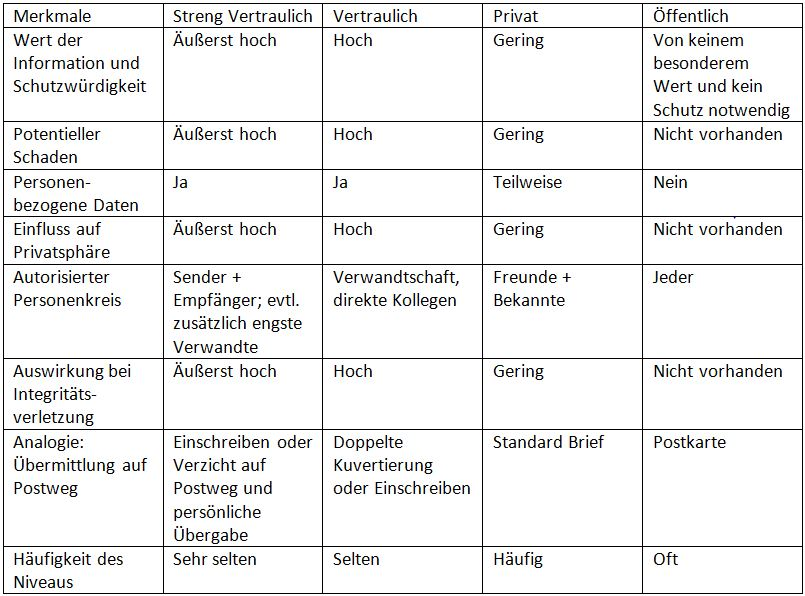
\includegraphics{sicherheitsniveaus.JPG}

Die \dots Abbildung 1 \dots im Tabellenkopf vier verschiedene Sicherheitsniveaus dar: Streng Vertraulich, Vertraulich, Privat und Öffentlich. Dabei nimmt das Sicherheitsbedürfnis sowie der Verschlüsselungsaufwand von Streng Vertraulich hin zu Öffentlich ab.
In der ersten Spalte sind verschiedene Merkmale aufgelistet, welche es dem Nutzer ermöglichen sollen, für eine ganz bestimmte Information ein geeignetes Sicherheitsniveau zu bestimmen.
Alle weiteren Felder enthalten die Ausprägung des Merkmals innerhalb des jeweiligen Sicherheitsniveaus.


Merkmale beschreiben

Ein Beispiel geben

